\setcounter{deso}{2}
\begin{name}
	{ÔN TẬP KIỂM TRA CUỐI HỌC KÌ 1 - tp2}
	{TOÁN 10}
	{LỚP TOÁN THẦY PHÁT}
	{\thoigian}
\end{name}
\Opensolutionfile{ans}[ans/10-CK1-Toan-tu-tam-De-3-Phan-1]
\TN
%Câu 1
\begin{ex}
 Dùng kí hiệu $\forall ,\exists $ để viết mệnh đề: "Tồn tại ít nhất một số thực có bình phương không dương".
\choice
{$\exists x\in \mathbb{R}\colon x^2\le 0$}
{$\exists x\in \mathbb{R}\colon x^2=0$}
{$\exists x\in \mathbb{R}\colon x^2<0$}
{$\forall x\in \mathbb{R}\colon x^2>0$}
\loigiai{ }
\end{ex}
%Câu 2
\begin{ex}
 Cặp số nào sau đây không phải là nghiệm của bất phương trình $5x-2(y-1)\le 0$?
\choice
{$(0;1)$}
{$(1;3)$}
{$(1;1)$}
{$(1;0)$}
\loigiai{ }
\end{ex}\newpage
%Câu 3
\begin{ex}
 Cho parabol $(P)\colon y=3x^2-2x+1$. Điểm nào sau đây là đỉnh của $(P)$?
\choice
{$I(0;1)$}
{$I\left(\dfrac{1}{3};\dfrac{2}{3}\right)$}
{$I\left(\dfrac{-1}{3};\dfrac{2}{3}\right)$}
{$I\left(\dfrac{1}{3};\dfrac{-2}{3}\right)$}
\loigiai{ }
\end{ex}
%Câu 4
\begin{ex}
 Hàm số nào sau đây là hàm số bậc hai?
\choice
{${y=x^3-2 x^2+5 x-7}$}
{${y=\dfrac{2022}{x^2+3 x-1}}$}
{${y=x^2-4 x+3}$}
{${y=\dfrac{1}{x^2}+\dfrac{3}{x}-1}$}
\loigiai{ }
\end{ex}\newpage
%Câu 5
\begin{ex}
 Tập nghiệm của bất phương trình $x^2-2 x+3>0$ là:
\choice
{${\varnothing}$}
{${\mathbb{R}}$}
{${(-\infty ;-1) \cup(3 ;+\infty)}$}
{${(-1 ; 3)}$}
\loigiai{ }
\end{ex}
%Câu 6
\begin{ex}
 Tam thức ${f(x)=x^2-(m+2) x+5 m+1}$ không âm với mọi $x\in R$ khi?
\choice
{${m>16}$}
{${0 \leq m \leq 16}$}
{${m<16}$}
{Không tồn tại $m$}
\loigiai{ }
\end{ex}\newpage
%Câu 7
\begin{ex}
 Tổng các nghiệm của phương trình $x-\sqrt{2x-4}=2$ là:
\choice
{$8$}
{$0$}
{$4$}
{$6$}
\loigiai{ }
\end{ex}
%Câu 8
\begin{ex}
 Số nghiệm của phương trình $\sqrt{x^2-2x-1}=\sqrt{-x^2+2x-1}$ là
\choice
{$1$}
{$0$}
{$2$}
{$3$}
\loigiai{ }
\end{ex}\newpage
%Câu 9
\begin{ex}
 Tính diện tích tam giác có ba cạnh lần lượt là $4$, $12$, $14$.
\choice
{$\dfrac{3}{2}\sqrt{55}$}
{$\sqrt{55}$}
{$165$}
{$3\sqrt{55}$}
\loigiai{ }
\end{ex}
%Câu 10
\begin{ex}
 Cho hình bình hành $ABCD$. Vectơ tổng $\vec{CB}+\vec{CD}$ bằng
\choice
{$\vec{DB}$}
{$\vec{BD}$}
{$\vec{AC}$}
{$\vec{CA}$}
\loigiai{ }
\end{ex}\newpage
%Câu 11
\begin{ex}
 Gọi $G$ là trọng tâm tam giác vuông $ABC~$ với cạnh huyền $BC = 12$. Vectơ $\vec{GB}-\vec{CG}$ có độ dài bằng
\choice
{$2$}
{$4$}
{$6$}
{$12$}
\loigiai{ }
\end{ex}
%Câu 12
\begin{ex}
 Cho tam giác $ABC$. Gọi $M$ là trung điểm của $AB$, $N$ là điểm thuộc $AC$ sao cho $\vec{CN}=2\vec{NA}$. $K$ là trung điểm của $MN$. Phân tích vectơ $\vec{AK}$ theo các vectơ $\vec{AB},\vec{AC}$.
\choice
{$\vec{AK}=\dfrac{1}{4}\vec{AB}+\dfrac{1}{6}\vec{AC}$}
{$\vec{AK}=\dfrac{1}{2}\vec{AB}+\dfrac{1}{3}\vec{AC}$}
{$\vec{AK}=\dfrac{1}{4}\vec{AB}+\dfrac{1}{3}\vec{AC}$}
{$\vec{AK}=\dfrac{1}{2}\vec{AB}+\dfrac{2}{3}\vec{AC}$}
\loigiai{ }
\end{ex}\newpage
\TNTF
%Câu 1
\begin{ex}
Cho hệ bất phương trình: $\heva{& x+2y-5\le 0 \\& 0\le x\le 3 \\& y\ge 0}$
\choiceTF
{Hệ bất phương trình đã cho là hệ bất phương trình bậc nhất hai ẩn}
{Điểm $A(1;-1)$ thuộc miền nghiệm của hệ bất phương trình đã cho}
{Miền nghiệm của hệ bất phương trình là hình chữa nhật}
{Biểu diễn miền nghiệm của hệ trên là một đa giác có diện tích bằng $5{,}25$}
\loigiai{ }
\end{ex}\newpage
%Câu 2
\begin{ex}
Cho tam thức bậc hai $f(x)=x^2-2mx-2m+3$
\choiceTF
{Với $m=1$, tam thức $f(x)$ có nghiệm $x=1$}
{Tam thức $f(x)$ có biệt thức $\Delta'=m^2+2m+3$}
{Tam thức $f(x)$ luôn dương với mọi $m\in (-3;1)$}
{Giả sử tam thức $f(x)$ có hai nghiệm phân biệt $x_1;x_2$, khi đó biểu thức $P=x_1^2+x_2^2+8x_1x_2$ đạt giá trị nhỏ nhất tại $m=\dfrac{3}{2}$}
\loigiai{ }
\end{ex}\newpage
%Câu 3
\begin{ex}
Cho $\Delta A B C$ có $AB=5,AC=4,\widehat{A}>90^\circ$, diện tích $S=5\sqrt{3}$.
\choiceTF
{$\sin A=\dfrac{\sqrt{3}}{2}$}
{$\cos A=\dfrac{-1}{2}$}
{$BC=\sqrt{62}$}
{$R=\sqrt{20}$}
\loigiai{ }
\end{ex}\newpage
%Câu 4
\begin{ex}
Cho tam giác $ABC$ đều cạnh bằng $a$, trọng tâm $G$, gọi $H$ là trung điểm $BC$.
\choiceTF
{$\vec{CA}-\vec{CB}=\vec{AB}$}
{$\vec{AB}+\vec{AC}=3\vec{AG}$}
{$\vec{GH}=\dfrac{1}{3}(\vec{AB}+\vec{AC})$}
{$\vec{CA} \cdot \vec{GC}=\dfrac{a^2}{2}$}
\loigiai{ }
\end{ex}\newpage

\TNSA
%Câu 1
\begin{ex}
 Cho tập hợp $A=\left\{ x\in \mathbb{Z}\left| |x-1|<3 \right. \right\}$. Có bao nhiêu tập hợp con của tập hợp $A$ có đúng $4$ phần tử?
 \shortans{6}
\loigiai{ }
\end{ex}
%Câu 2
\begin{ex}
Cho hàm số $y=ax^2+bx+2$ có bảng biến thiên như hình vẽ sau đây.
\begin{center}

\begin{tikzpicture}
\tkzTabInit[lgt=2,espcl=3]
{$x$/1,$y$/2}
{$-\infty$,$\dfrac{3}{2}$,$+\infty$}

\tkzTabVar
{+/$+\infty$, -/$-\dfrac{1}{4}$, +/$+\infty$}

\end{tikzpicture}
\end{center}
Tính giá trị biểu thức $A=a+b$.
\shortans{4}
\loigiai{ }
\end{ex}\newpage
%Câu 3
\begin{ex}
 Một viên gạch hình vuông có cạnh thay đổi được đặt nội tiếp trong một hình vuông có cạnh bằng $20\,cm$, tạo thành bốn tam giác xung quanh như hình vẽ. Tính tổng tất cả các giá trị nguyên của $x$ để diện tích viên gạch không vượt quá $208\,cm^2$.
\begin{center}
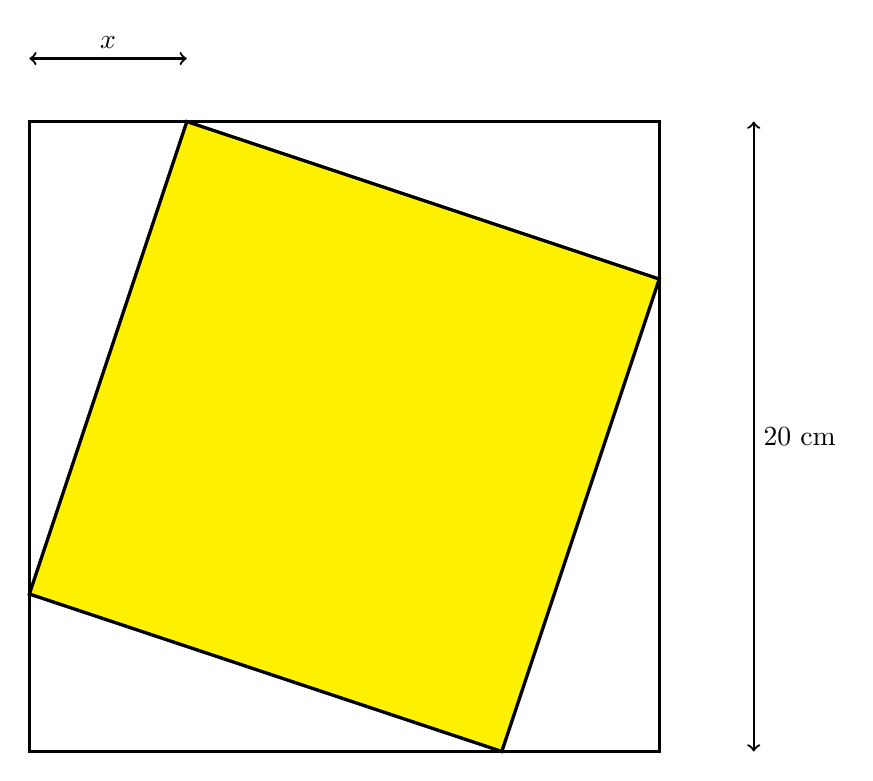
\begin{tikzpicture}[scale=0.4]

% Tham số
\def\a{20}   % cạnh hình vuông lớn
\def\x{5}    % độ lệch x (có thể thay đổi)

% Hình vuông lớn
\draw[line width=1.2pt]
(0,0) rectangle (\a,\a);

% Các điểm của hình vuông nghiêng
\coordinate (A) at (\x,\a);
\coordinate (B) at (\a,\a-\x);
\coordinate (C) at (\a-\x,0);
\coordinate (D) at (0,\x);

% Hình vuông nghiêng
\fill[yellow] (A)--(B)--(C)--(D)--cycle;
\draw[line width=1.2pt] (A)--(B)--(C)--(D)--cycle;

% Mũi tên chỉ x
\draw[<->, thick]
(0,\a+2) -- (\x,\a+2);
\node[above] at (\x/2,\a+2) {$x$};

% Mũi tên chỉ 20 cm
\draw[<->, thick]
(\a+3,0) -- (\a+3,\a);
\node[right] at (\a+3,\a/2) {20 cm};

\end{tikzpicture}
\end{center}
\shortans{36}
\loigiai{ }
\end{ex}\newpage
%Câu 4
\begin{ex}
 Một chú thỏ ngày nào cũng ra bờ suối ở vị trí $A$, cách cửa hang của mình tại vị trí $B$ là $370~m$ để uống nước, sau đó chú thỏ sẽ đến vị trí $C$ cách vị trí $A$ là $120~m$ để ăn cỏ rồi trở về hang. Tuy nhiên, hôm nay sau khi uống nước ở bờ suối, chú thỏ không đến vị trí $C$ như mọi ngày mà chạy đến vị trí $D$ để tìm cà rốt rồi mới trở về hang (xem hình bên dưới). Biết rằng, tổng thời gian chú thỏ chạy từ vị trí $A$ đến vị trí $D$ rồi về hang là 30 giây (không kể thời gian tìm cà rốt), trên đoạn $AD$ chú thỏ chạy với vận tốc là $13~m/s$, trên đoạn $BD$ chú thỏ chạy với vận tốc là $15~m/s$. Vị trí $C$ cách vị trí $D$ bao nhiêu mét?
\begin{center}
\begin{tikzpicture}[scale=0.3, line cap=round, line join=round]

% Các điểm
\coordinate (A) at (0,0);
\coordinate (C) at (0,12);
\coordinate (D) at (12,12);
\coordinate (B) at (37,12);

% Các đoạn thẳng
\draw[thick] (A)--(C)--(B);
\draw[thick] (A)--(B);
\draw[thick] (A)--(D);

% Góc vuông tại C
% \draw (C) ++(0,-.8) -- ++(.8,0) -- ++(0,.8);

% Mũi tên chỉ hướng
% \draw[->, thick] (D) -- ++(6,0);
% \draw[->, thick] ($(A)!0.4!(D)$) -- ++(1.5,2.5);

% Ghi độ dài
\node[left] at ($(A)!0.5!(C)$) {120 m};
\node[below] at ($(A)!0.5!(B)$) {370 m};

% Nhãn các điểm
\node[below left] at (A) {A};
\node[above left] at (C) {C};
\node[above] at (D) {D};
\node[above right] at (B) {B};

\end{tikzpicture}
\end{center}
\shortans{50}
\loigiai{ }
\end{ex}\newpage
%Câu 5
\begin{ex}%[0-HK1-KN-7-HaDong-HaNoi-2324]%[VN-MT-6, Đoàn Thị Lý]%[0H9V2-3]
Trong mặt phẳng tọa độ $Oxy$ cho các điểm $A(1;7)$, $B(-2;3)$. Điểm $M(a;0)$ trên $Ox$ sao cho $M$ cách đều $A$, $B$. Tính $a$ (kết quả để ở dạng thập phân, làm tròn đến hàng phần trăm).
\shortans{$6{,}17$}
\loigiai{
Ta có $MA=MB\Leftrightarrow\sqrt{(1-a)^2+7^2}=\sqrt{(-2-a)^2+3^2}\Leftrightarrow 6a-37=0\Leftrightarrow a=\dfrac{37}{6}\approx 6{,}17$.
}
\end{ex}\newpage
%Câu 6
\begin{ex}
 Cho ba lực $\vec{F_1}=\vec{MA},\vec{F_2}=\vec{MB},\vec{F_3}=\vec{MC}$ cùng tác động vào một vật tại điểm M và vật đứng yên như hình vẽ. Biết cường độ của lực $\vec{F}_3$ là $50\sqrt{3}N$, $\widehat{AMB}=120^\circ,\widehat{AMC}={{150}^\circ}$. Tìm cường độ của lực $\vec{F_1}$.
\shortans{100}
\loigiai{ }
\end{ex}\newpage
\Closesolutionfile{ans}